\chapter{Solution d'allocation de ressources dans un environnement \emph{Fog Computing}: Stable Matching based Resources Allocation (SMRA)}

\section{Introduction}
Nous avons vu à travers le chapitre précédent que le Fog Computing est caractérisé par l'homogéniété de ses composants materiels et des requêtes y circulant. D'où le besoin d'une technique de gestion efficace permettant d'établir une correspondance entre les demandes des Objets IoT et les ressources disponibles.\par
Nous définirons dans ce chapitre les concepts sur lesquels repose note solution, et puis nous présenterons les algorithmes qui la composent et son scénario d'exécution nominal.

\section{Motivation}
Une bonne gestion de ressources permet d'accroître les performances globales du système, en réduisant le temps d'exécution des différentes applications, la latence, ainsi que les coûts énergétiques. Elle permet aussi d'exploiter au mieux les ressources matérielles disponibles, ce qui augmente le rendement et la rentabilité économique des différents équipements.\\ 
Par conséquent, le développement d'un bon modèle de gestion de ressource se révèle d'une importance capitale pour une exploitation efficace et rentable d'une infrastructure Fog.

\section{Problématique et article de référence}
Suite à l'étude des travaux qui traitent de l'amélioration et de l'optimisation de la gestion des ressources, on constate que le problème de planification des ressources est un problème central qui nécessite d'être investigué afin d'effectuer une gestion de ressources optimale. \\
Le problème consiste à concevoir un modèle de planification de ressources dynamique, efficace et évolutif, qui permet d'affecter les différentes demandes de ressources, effectuées par les appareils IoT, aux différents nœuds Fog d'une manière à optimiser au mieux certaines métriques liées aux coûts.\\
Pour la réalisation de ce travail, nous nous sommes inspirés d'un article publié traitant une problématique similaire \cite{jing2016}. \\
Dans ce travail, les auteurs s'intéressent au processus d'approvisionnement dans un environnement \emph{Cloud}, dans lequel ce processus peut être principalement décomposé en 3 étapes majeures à savoir : 
\begin{enumerate}
    \item L'identification des nœuds concernés (c.-à-d. les nœuds sous-utilisés ou sur-utilisés). 
    \item Sélection des VMs à migrer.
    \item Réallocation des VMs aux nœuds sous-utilisés.
\end{enumerate}
La partie qui nous intéresse est la troisième étape où ils proposent un mécanisme d'affectation de VMs aux nœuds adéquat, modélisé comme étant un problème de correspondance (matching problem).

\section{Conception de la solution}
\subsection{Contribution}
Dans notre solution, nous proposons une nouvelle technique l'allocation des nœuds d'un environnement Fog afin de mieux servir les requêtes générés par les objets \emph{IoT}, cette technique se base sur une implémentation de l'algorithme de gale-shapley \cite{gale-shapley} (Stable Matching based Resources Allocation ou SMRA) et elle est détaillée dans ce qui suit.\par

\subsubsection{Hypothèses}
Afin de pouvoir se focaliser sur le problème de correspondance entre les demandes de services et les nœuds Fog, et à cause des limites de l'envrionnement de simulation, nous devons d'abord formuler certaines hypothèses sur la topologie physique de l'infrastructure Fog.\\
\begin{itemize}
    \item La topologie est statique durant l'exploitation: une fois la solution implémentée, la topologie ne subit pas de modification.
    \item La topologie suit une organisation matricielle: les nœuds Fog sont organisés en des niveaux bien distincts avec le même nombre de nœuds dans chaque niveau.
    \item La topologie est maillée entre les niveaux: chaque nœud Fog du cluster est relié physiquement à tous les nœuds du niveau supérieur.
    \item Chaque nœud à une connaissance de tous ses nœuds parents et ses nœuds enfants (c.-à-d. respectivement les nœuds du niveau supérieur et les nœuds du niveau inférieur)
    \item Dans ce modèle, nous disposons au minimum de trois types de requêtes qui sont : \\
          \begin{itemize}
             \item La requête \emph{demande}, qui correspond à une demande de services émise par les appareils IoT, elle comporte tous les détails de la demande.
             \item la requête \emph{résultat}, qui est généré après l'exécution d'une demande de service, elle est émise à destination de l'objet \emph{IoT} émetteur.
             \item La requête \emph{jeton}, qui représente le jeton circulant entre les différents nœuds passerelle suivant la politique du tourniquet (round-robin).
          \end{itemize}
\end{itemize}

SMRA se décompose en 4 aspects interdépendants que nous détaillons par la suite: 
\begin{description}
  \item[La clusterisation:] en regroupant les nœuds Fog dans des groupe (Cluster) de par leur proximité géographique.
  \item[le profiling:] en attribuant des différents profiles ou rôles aux différents nœuds d'un cluster.
  \item[La traîtement par lôt (Batch Computin):] les demandes sont regroupées et traitées par lôt selon leurs ordres d'arrivée.
  \item[Le matching:] le processus de correspondance et de redirection des demandes vers les neouds Fog adéquats.
\end{description}

\subsection{Topologie}
Comme vu dans le chapitre introductif, une infrastructure \emph{Fog} classique est décomposée de 3 couches superposées qui sont (voir Figure \ref{fig:Topologie_generale_de_linfrastructure}) :
\begin{itemize}
    \item \emph{La couche IoT}, qui représente l'ensemble des objets \emph{IoT} qui effectue des demandes de service.
    \item \emph{La couche Fog}, qui représente l'ensemble des nœuds \emph{Fog} se trouvant à l'intermédiaire entre les objets \emph{IoT} et le \emph{cloud}.
    \item \emph{La couche Cloud} qui représente l'infrastructure Cloud traditionnelle.
\end{itemize}
\begin{figure}[H]
    \centering
    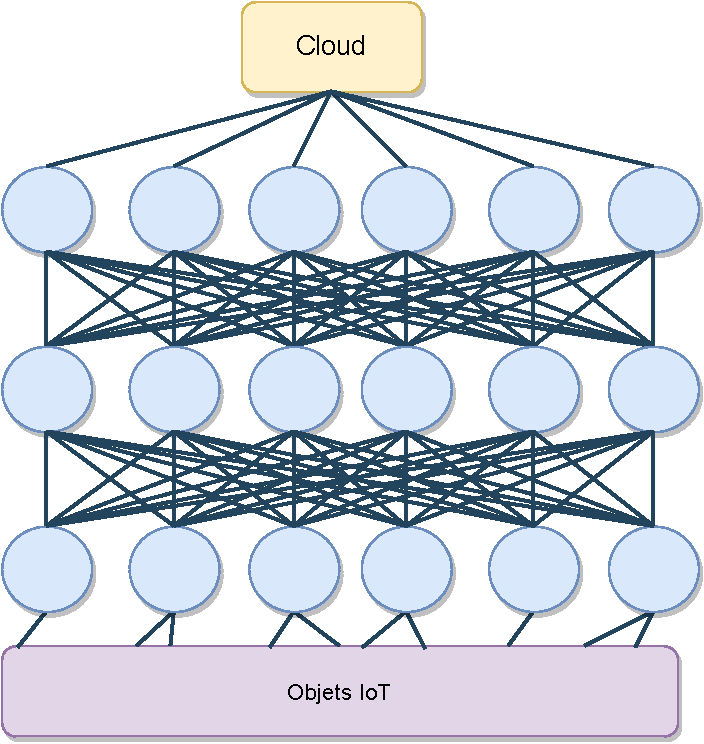
\includegraphics[]{Topologie_générale_de_l'infrastructure.pdf}
    \caption{Schémas représentant une architecture Fog traditionnelle}
    \label{fig:Topologie_generale_de_linfrastructure}
\end{figure}
SMRA commence par découper verticalement la couche \emph{Fog} de l'infrastructure en un ensemble de clusters\footnote{Nous discutons des critères de scalabilité verticale et horizontale du cluster dans le chapitre suivant, où nous montrons les résultats obtenus par rapport à différentes dimensions du cluster.} (voir Figure \ref{fig:Infrastructure_fog_repartie_en_cluster}) , c.-à-d. chaque cluster regroupe un ensemble de nœuds \emph{Fog} inter-connecté. Ensuite, chaque cluster est découpé en 2 couches superposées, qui sont :
\begin{itemize}
    \item \emph{La couche des nœuds passerelles :}  cette couche est composée du niveau connecté directement à la couche \emph{IoT}.
    \item \emph{La couche des nœuds Fog restants :} qui est composée des niveaux intermédiaires restants entre la couche des nœuds passerelles et le \emph{cloud}.
\end{itemize}
\begin{figure}[H]
    \centering
    \includegraphics[scale=0.8]{ShémaCluster.pdf}
    \caption{Schéma représentant une architecture \emph{Fog} répartie en clusters}
    \label{fig:Infrastructure_fog_repartie_en_cluster}
\end{figure}

\subsection{Scénario}
Ce scénario s'applique pour un cluster, puisque les clusters sont indépendants, il suffit par la suite de généraliser ce fonctionnement à l'ensemble des clusters défini par l'infrastructure.\par
Les nœuds passerelles du cluster, reçoivent des demandes de services des différents appareils IoT. Chaque nœud préserve ses demandes dans une file en attendant leur correspondance puis leur envoi à leur destination.\par
Nous définissons un jeton circulant d'un nœud passerelle à un autre suivant la politique du tourniquet (round robin). Si un nœud passerelle possède le jeton à la réception alors il effectue une correspondance des demandes qui se trouve dans sa file d'attente avec les nœuds \emph{Fog} du cluster, puis il envoie chaque demande au nœud \emph{Fog} correspondant, et  renvoie le jeton au prochain nœud passerelle et ainsi de suite (voir Figure \ref{fig:Organigrame_scénario_globale}).

\subsection{Description algorithmique du scénario}
SMRA est conçu suivant le paradigme événementiel, c.-à-d. une approche algorithmique basée sur la notion d'événement, où on cherche à associer à chaque événement une procédure à exécuter appelée “Routine”.   
SMRA comporte 2 routines principales qui sont :
\begin{itemize}
    \item \emph{La Routine associée aux nœuds passerelles}
    \item \emph{La Routine associée au nœud Fog restants}
\end{itemize}

\subsubsection{Routine associée aux nœuds passerelles}
Cette routine est exécutée au niveau des nœuds passerelles à chaque fois qu'une requête est reçue.
Le pseudo-code de cette routine est le suivant :\\
\begin{algorithm}[H]
  \KwData{ListeDemandes, ListeNoeuds}
  \eIf{Requête reçue est de type jeton}
  {  
    \emph{// appeler la  procédure Correspondance.}\\
    correspondance(fileDemandes, listeNoeuds);\\
    \emph{// puis on effectue le routage des demandes.}\\
    \ForEach{Demande $D_i \in fileDemandes$}
    {
      \eIf{listeParents.contient($D_i$.destination)}
      {
        envoyer(demande, $D_i$.destination);
      }
      {
        envoyer(demande, NoeudPèreParDéfaut);\\
        \emph{// on met à jour le nœud par défaut à chaque fois afin d'équilibrer la charge entre les différentes liaisons.}\\
        NoeudPèreParDéfaut $\gets$ prochainNoeudParent();\\
      }
    }
  }
  {
    \eIf{Requête reçue est de type résultat}
    {
      \emph{// envoyer le résultat à l'appareil IoT concerné.}\\
      envoyer(resultat, resultat.destination);
    }
    {
      \emph{// la requête est par conséquent de type demande.}\\
      enfiler(fileDemandes, Demande);
    }
  }
  \caption{Routine associée aux nœuds passerelles}
\end{algorithm}
\\
\paragraph{Procédure de correspondance :}
Pour l'implémentation de cette procédure, nous avons opté pour l'utilisation de l'algorithme de Gale-Shapley \cite{gale-shapley}, qui est un algorithme conçu pour résoudre le problème des mariages stables.\\
Il présente des propriétés intéressantes qui sont :
\begin{itemize}
  \item De bonne performance due à sa complexité quadratique ($\mathcal{O}(n^2)$).
    \item Convergence: toute demande sera associée à un nœud à la fin de l'exécution.
    \item Les couples (demande,nœud) résultant de cet algorithme sont stables (voir Annexe).
    \item La configuration résultante est optimale en comparaison à toutes les autres solutions stables \cite{gale-shapley}.
\end{itemize} \\
Cet algorithme nécessite la définition d'une relation de préférence, que nous nommerons "Relation d'adéquation" ou RA qui est associée à chaque demande et à chaque nœud:\\
Pour ce faire, nous définissons une distance entre la demande et le nœud, qui est calculé de la manière suivante :
\\ \\
\begin{minipage}[t]{0.4\textwidth}
\begin{flushleft}
    \begin{tabular}{| c | p{4cm}|}
    \hline
    Symbole & Définition \\
    \hline
    $C_u$ & MIPS\footnote{million d'instructions par seconde} utilisé \\ 
    \hline
    $C_{dem}$ & MIPS exigés par le service à exécuter \\
    \hline
    $C_fd$ & MIPS totale du nœud \\
    \hline
    $C_r$ & MIPS disponible \\
    \hline
    \end{tabular}
\end{flushleft}
\end{minipage}
%
\begin{minipage}[th]{0.4\textwidth}
\begin{flushright} 
\begin{center}
    $$Distance =\left \lbrace 
    \begin{array}{ll}
        \frac{C_u + Cdem}{C_fd}/ & \mbox{si $C_r > C_{dem}$}\\
        -1 & \mbox{sinon}
    \end{array}
\right.$$
\end{center}
\end{flushright}
\end{minipage}
\\ \\ \\
La relation d'adéquation est définie par la distance minimale entre le nœud et la demande.\\
Autrement dit, soit $D=\{D_1,D_2,..,D_n\}$ un ensemble de demandes, et soit $N=\{N_1,N_2,..,N_n\}$.\\
On dit que le nœud $N_j$ est le mieux adéquat à la demande $D_i$ ssi : \\
$Distance(D_i,N_j) = Min (Distance(D_i,N_m)), \forall m \in \{1,..,n\}$. \\
\textbf{Pseudo-code de la procédure :}\\
\begin{algorithm}[H]
  \KwData{ListeDemandes, ListeNoeuds}
  \emph{// initialisation de toutes les demandes à une destination null.}\\
  \ForEach{Demande $D_i \in ListeDemandes$}
  {
    $D_i$.destination $\gets$ null;\\
  }
  \While{$\exists$ une\ demande\ $d$\ non\ affectée\ qui\ peut\ se\ proposer\ à\ un\ nœud}
  {
    %n $\gets$ le\ nœud\ le\ mieux\ adéquat\ à\ $d$\ parmi\ la\ liste\ des\ nœuds\ auquel\ $d$\ ne\ s'est\ pas\ déjà\ proposé;\\
    n $\gets$ le\ nœud\ le\ mieux\ adéquat\ à\ $d$\ telque\ $d$\ \notin\ $nœud.demandesRejetées$;\\
    \eIf{$n$ = null}
    {
      \emph{// si aucun nœud ne peut traiter la demande, elle est déléguée au cloud.}\\
      d.destination $\gets$ cloud;\\
      envoyerVersCloud(d);\\
    }
    {
      \eIf{$n$ est libre}
      {
        d.destination $\gets$ n;\\
      }
      {
        \emph{// si le nœud n'est pas libre et que $d$ est plus adéquate que la demande associée à n.}\\
        \eIf{distance(n,n.demande) > distance(n,d)}
        {
          \emph{// la destination de la demande associée à n est remise à null pour qu'elle soit retraiter.}\\
          n.demande.destination $\gets$ null;\\
          \emph{// puis elle est ajoutée aux demandes rejetées par le nœud pour qu'elle ne puisse pas se reproposer.}  \\
          n.demandesRejetées.ajouter(n.demande);\\
          \emph{// la demande associée à n est remplacée par d.}\\
          n.demande $\gets$ d;\\
          d.destination $\gets$ n;\\
        }
        {
          \emph{// la demande d a été rejetée par le nœud donc elle ne peut plus se reproposer.}\\
          n.demandesRejetées.ajouter(d);\\
        }
      }
    }
  }
  \caption{Procédure de correspondance}
\end{algorithm}

\subsubsection{Routine associée au nœud Fog :}
Cette routine est exécutée au niveau des nœuds Fog à chaque fois qu'une requête est reçue.\\
\textbf{Pseudo-code de la routine :}\\
\begin{algorithm}[H]
  %\KwData{this text}
  %\KwResult{how to write algorithm with \LaTeX2e }
  \eIf{Requête reçue est de type demande}
  {  
    \eIf{demande.destination correspond au nœud lui-même}
    { 
      \emph{// la destination du résultat et la source de la demande.}\\
      resultat $\gets$ executer(demande);\\
      \emph{// puis effectuer le routage du résultat.}\\
      \eIf{listeEnfants.contient(resultat.destination)}
      {
        envoyer(resultat, resultat.destination);\\
      }
      {
        envoyer(resultat, NoeudFilsParDefaut);\\
        NoeudFilsParDéfaut $\gets$ prochainNoeudFils();\\
      }
    }
    {  
      \emph{// le nœud en question n'est pas la destination.}\\
      \eIf{listeParents.contient(demande.destination)}
      {
        envoyer(demande, demande.destination);\\
      }
      {
        envoyer(demande,NoeudPèreParDéfaut);\\
        NoeudPereParDéfaut $\gets$ prochainNoeudParent();\\
      }
    }
  }
  {
    \emph{// la requête reçue est par conséquent une requête résultat.}\\
    \eIf{listeEnfants.contient(resultat.destination)}
    {
      envoyer(resultat, resultat.destination);\\
    }
    {
      envoyer(resultat, NoeudFilsParDefaut);\\
      NoeudFilsParDéfaut $\gets$ prochainNoeudFils();\\
    }
  }
  \caption{Routine associée aux nœuds passerelles}
\end{algorithm}
\begin{figure}[H]
    \centering
    \includegraphics[]{Organigramme-scénario-globale.pdf}
    \caption{Organigramme du scénarion d'exécution du SMRA}
    \label{fig:Organigrame_scénario_globale}
\end{figure}

\section{Conclusion}
Dans ce chapitre, nous avons présenté notre solution en introduisant les entités interagissantes de notre environnement tout en formulant certaines hypothèses sur ce dernier. Nous décrivons aussi le scénario nominal d'exécution et nous détaillons les algorithmes exploités à chaque niveau.\par
Dans le prochain chapitre, nous passerons à l'étape d'implémentation de la solution sur une plateforme de simulation d'environnement Fog, et nous finirons par une discussion des résultats obtenus.
